\chapter{Implementacija i korisničko sučelje}
		
		
		\section{Korištene tehnologije i alati}
		
		Komunikacija u timu ostvarena je korištenjem aplikacija \underline{Whatsapp}\footnote{\url{https://www.whatsapp.com}} i \underline{Discord}\footnote{\url{https://discord.com}}. 
		Za upravljanje izvornim kodom korišten je sustav \underline{Git}\footnote{\url{https://git-scm.com}}, a udaljeni repozitorij dostupan je na web platformi \underline{GitLab}\footnote{\url{https://about.gitlab.com}}. 
		Za izradu UML dijagrama iskoristili smo alat \underline{Astah}\footnote{\url{https://astah.net}}.

		Razvojno okruženje korišteno u Android dijelu aplikacije je \underline{Android Studio}\footnote{\url{https://developer.android.com/studio}} - integrirano 
		razvojno okruženje (IDE) kreirano na temeljima drugog JetBrainsovog IDE-a, IntelliJa. Također službeni je Googleov IDE za razvoj Android aplikacija, a rad u njemu je moguć
		u sva tri glavna operacijska sustava (Windows, Linux, MacOS).
		
		Za backend dio programskog koda korišten je Microsoftov uređivač teksta \underline{Visual} \underline{Studio} \underline{Code}\footnote{\url{https://code.visualstudio.com}}. 
		Iako je samo uređivač teksta,
		VSC, zahvaljujući mnoštvu plugina razvijenih od programerske zajednice, podsjeća na razvojno okruženje. U njemu je integriran i sustav Git što nam je olakšalo rad.

		Aplikacija je napisana za Android operacijski sustav s podrškom za verzije 10, 11, 12 koristeći programski jezik \underline{Kotlin}\footnote{\url{https://kotlinlang.org}}, 
		a cloud funkcije za bazu podataka Firebase pisane su u \underline{Node.js}\footnote{\url{https://nodejs.org}}, \underline{Javascript}\footnote{\url{https://www.javascript.com}}
		frameworku za izradu backenda. Node.js vrti se na V8 engineu te izvršava JavaScript kod izvan preglednika. Primarno služi za razvoj serverske strane web stranica
		za prikazivanje dinamičkog sadržaja, ali može poslužiti u bilo kojem dijelu serverskog programiranja. 

		Baza podataka se nalazi na Googleovom poslužitelju i razvijana je pomoću \underline{Firebase}\footnote{\url{https://firebase.google.com}} Google platforme.
		Firebase se koristi za praćenje analitike, prijavljivanje i popravljanje rušenja aplikacija, a ima ugrađene baze podataka (Realtime i Firestore).

		Unit testiranje smo vršili pomoću \underline{Mockito}\footnote{\url{https://site.mockito.org}} \textit{frameworka} koji je razvijan pod MIT licencom. Programski jezik korišten
		za testiranje je Kotlin.
		
			
			\eject 
		
	
		\section{Ispitivanje programskog rješenja}
			
			\subsection{Ispitivanje komponenti}
			\justify{Napravljena su 4 testa za AuthenticationViewModel:\newline
			\textbf{loginFakeUser()} provjerava error handling za pokušaj prijave nepostojećeg korisnika\newline
			\textbf{loginEmptyEmail()} provjerava error handling za pokušaj prijave s praznim email-om\newline
			\textbf{registerEmptyEmail()} provjerava error handling za pokušaj registracije s praznim email-om\newline
			\textbf{logout()} provjerava error handling za pokušaj odjave bez prijavljenog korisnika}
			
			\begin{figure}[H]
				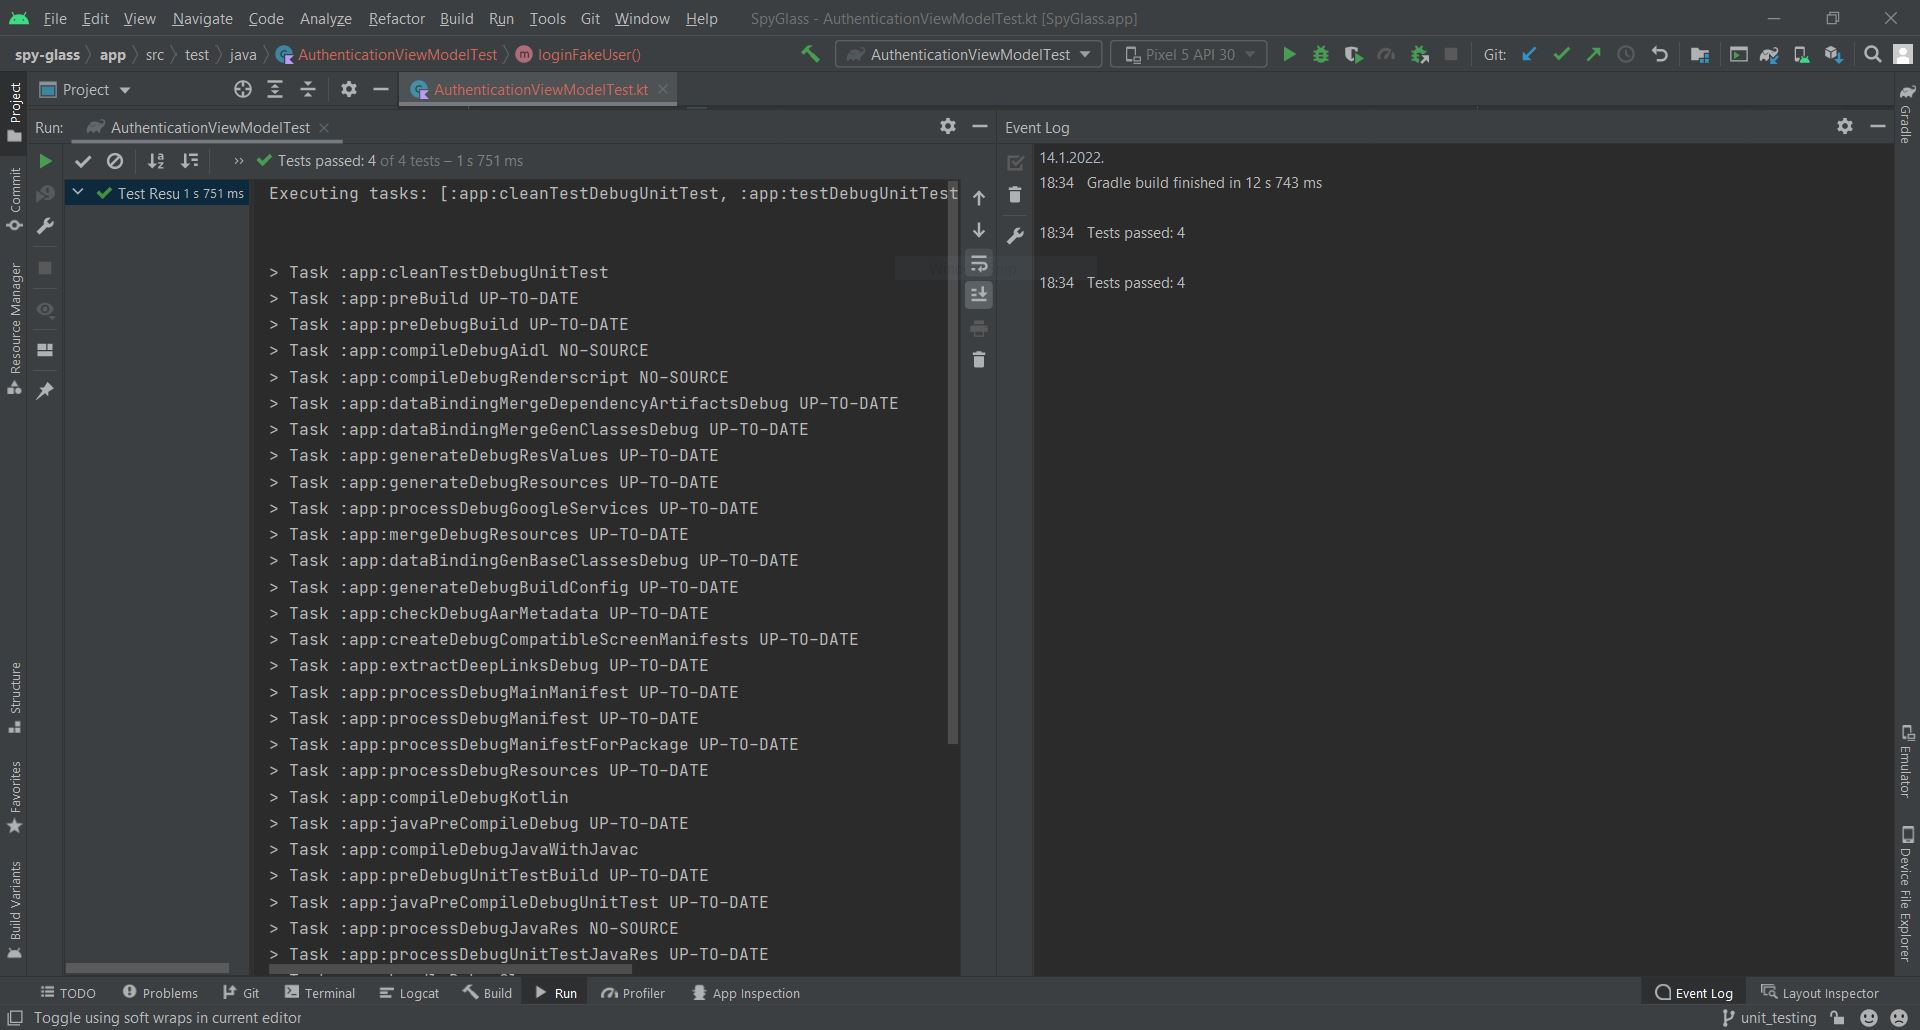
\includegraphics[width=\textwidth]{slike/testResultsAuth.jpg}
				\caption{Rezultati testova - AuthenticationViewModelTests}
			\end{figure}
			
			\begin{figure}[H]
				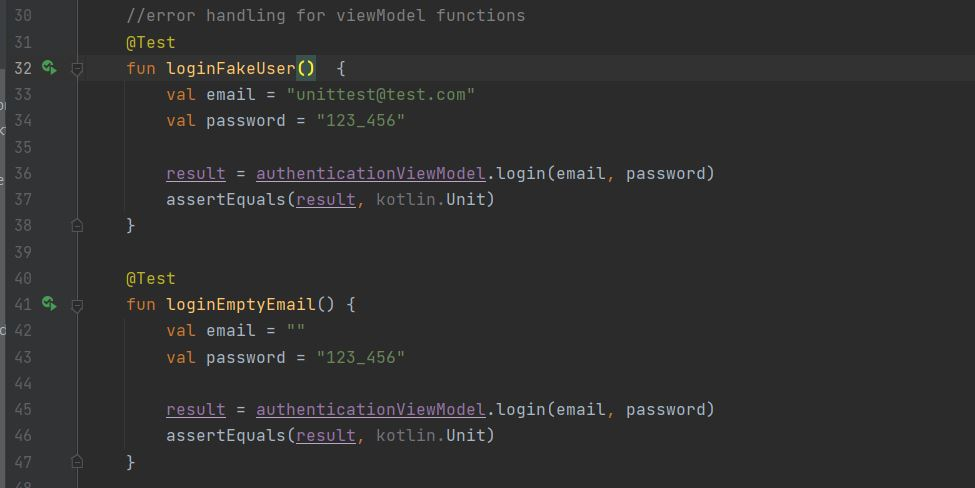
\includegraphics[width=\textwidth]{slike/authTests1.jpg}
				\caption{Isječak koda - AuthenticationViewModelTests}
			\end{figure}
			
			\begin{figure}[H]
				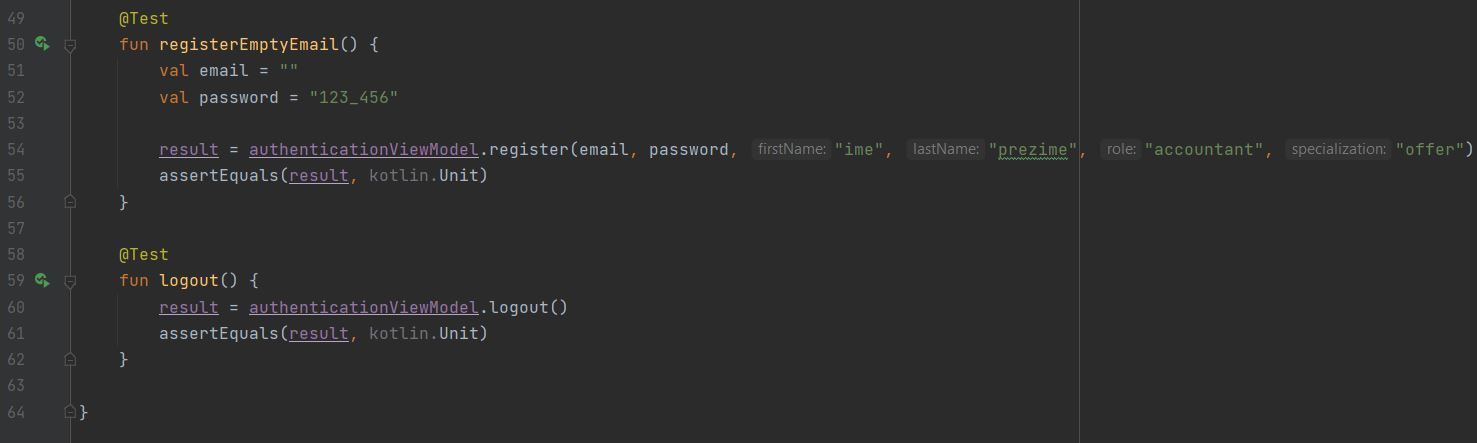
\includegraphics[width=\textwidth]{slike/authTests2.jpg}
				\caption{Isječak koda - AuthenticationViewModelTests}
			\end{figure}
			
			\justify{Napravljena su 2 testa za DocumentsViewModel:\newline
			\textbf{getDocumentsByFakeUser()} provjerava error handling za pokušaj dohvata dokumenata nepostojećeg korisnika\newline
			\textbf{getDocumentsLiveDataTest()} provjerava inicijalizaciju varijable documentsLiveData: MutableLiveData\textless List\textless Document\textgreater \textgreater}\\
			
			\begin{figure}[H]
				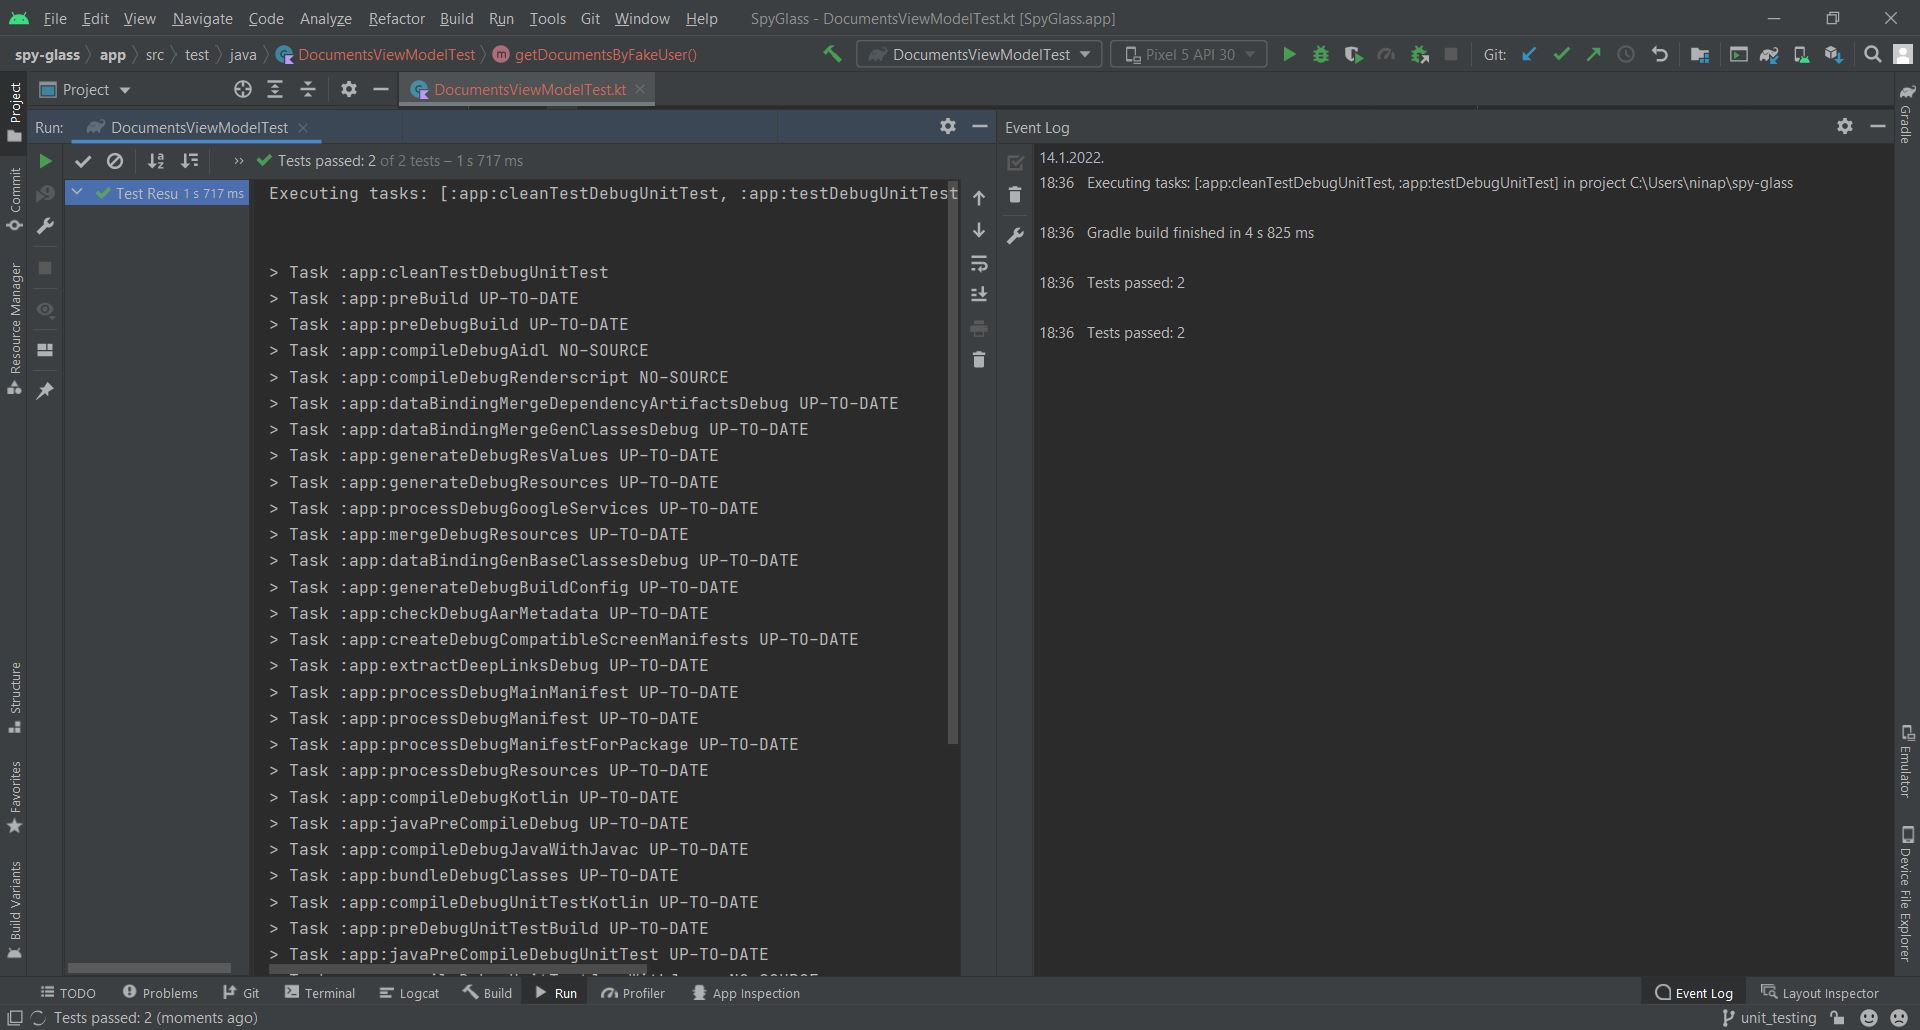
\includegraphics[width=\textwidth]{slike/testResultsDocs.jpg}
				\caption{Rezultati testova - DocumentsViewModelTests}
			\end{figure}
			
			\begin{figure}[H]
				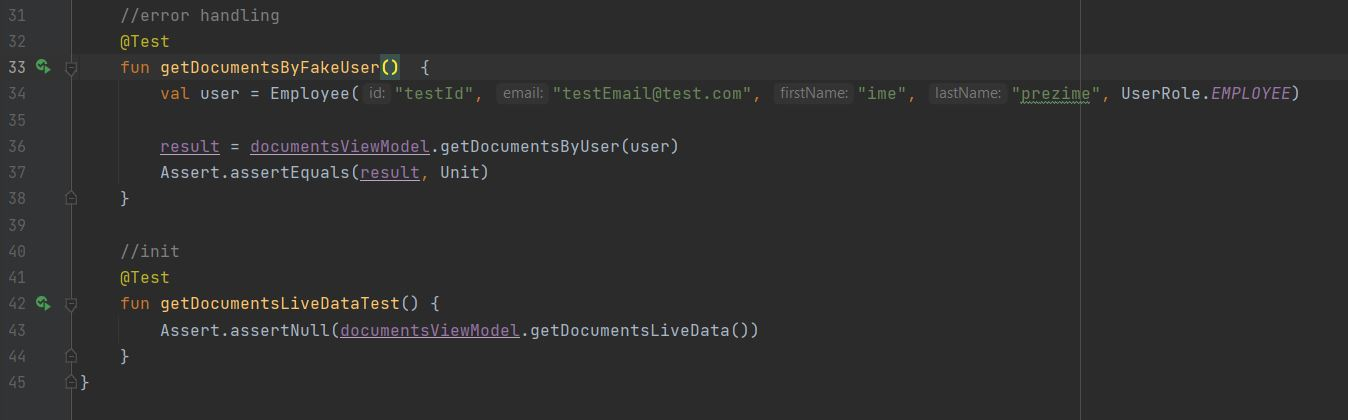
\includegraphics[width=\textwidth]{slike/documentsTests.jpg}
				\caption{Isječak koda - DocumentsViewModelTests}
			\end{figure}
			
			\subsection{Ispitivanje sustava}
			\justify{Svaki dio sustava ispitan je ručno po obrascima uporabe kako bi se pronašla neočekivana ponašanja aplikacije. Prikazan je dio ispitivanja sustava zbog jednostavnosti (UC1 - Registracija).
			\newline
			\newline
			\newline
			\textbf{Ispitni slučaj 1: Ispitivanje registracije direktora\newline
			Ulaz:\newline}
			1. Otvaranje aplikacije\newline
			2. Upisivanje identifikacijskih podataka\newline
			3. Pritiskanje gumba za registraciju 
			\newline
			\textbf{Očekivani rezultat:}
			\newline
			1. Prikazuje se zaslon za registraciju\newline
			2. Provjera formata unosa\newline
			3. Pošalji podatke i prihvati registraciju
			\newline
			\textbf{Rezultat: } Očekivanja su zadovoljena. Aplikacija je prošla test.
			}
			\begin{figure}[H]
				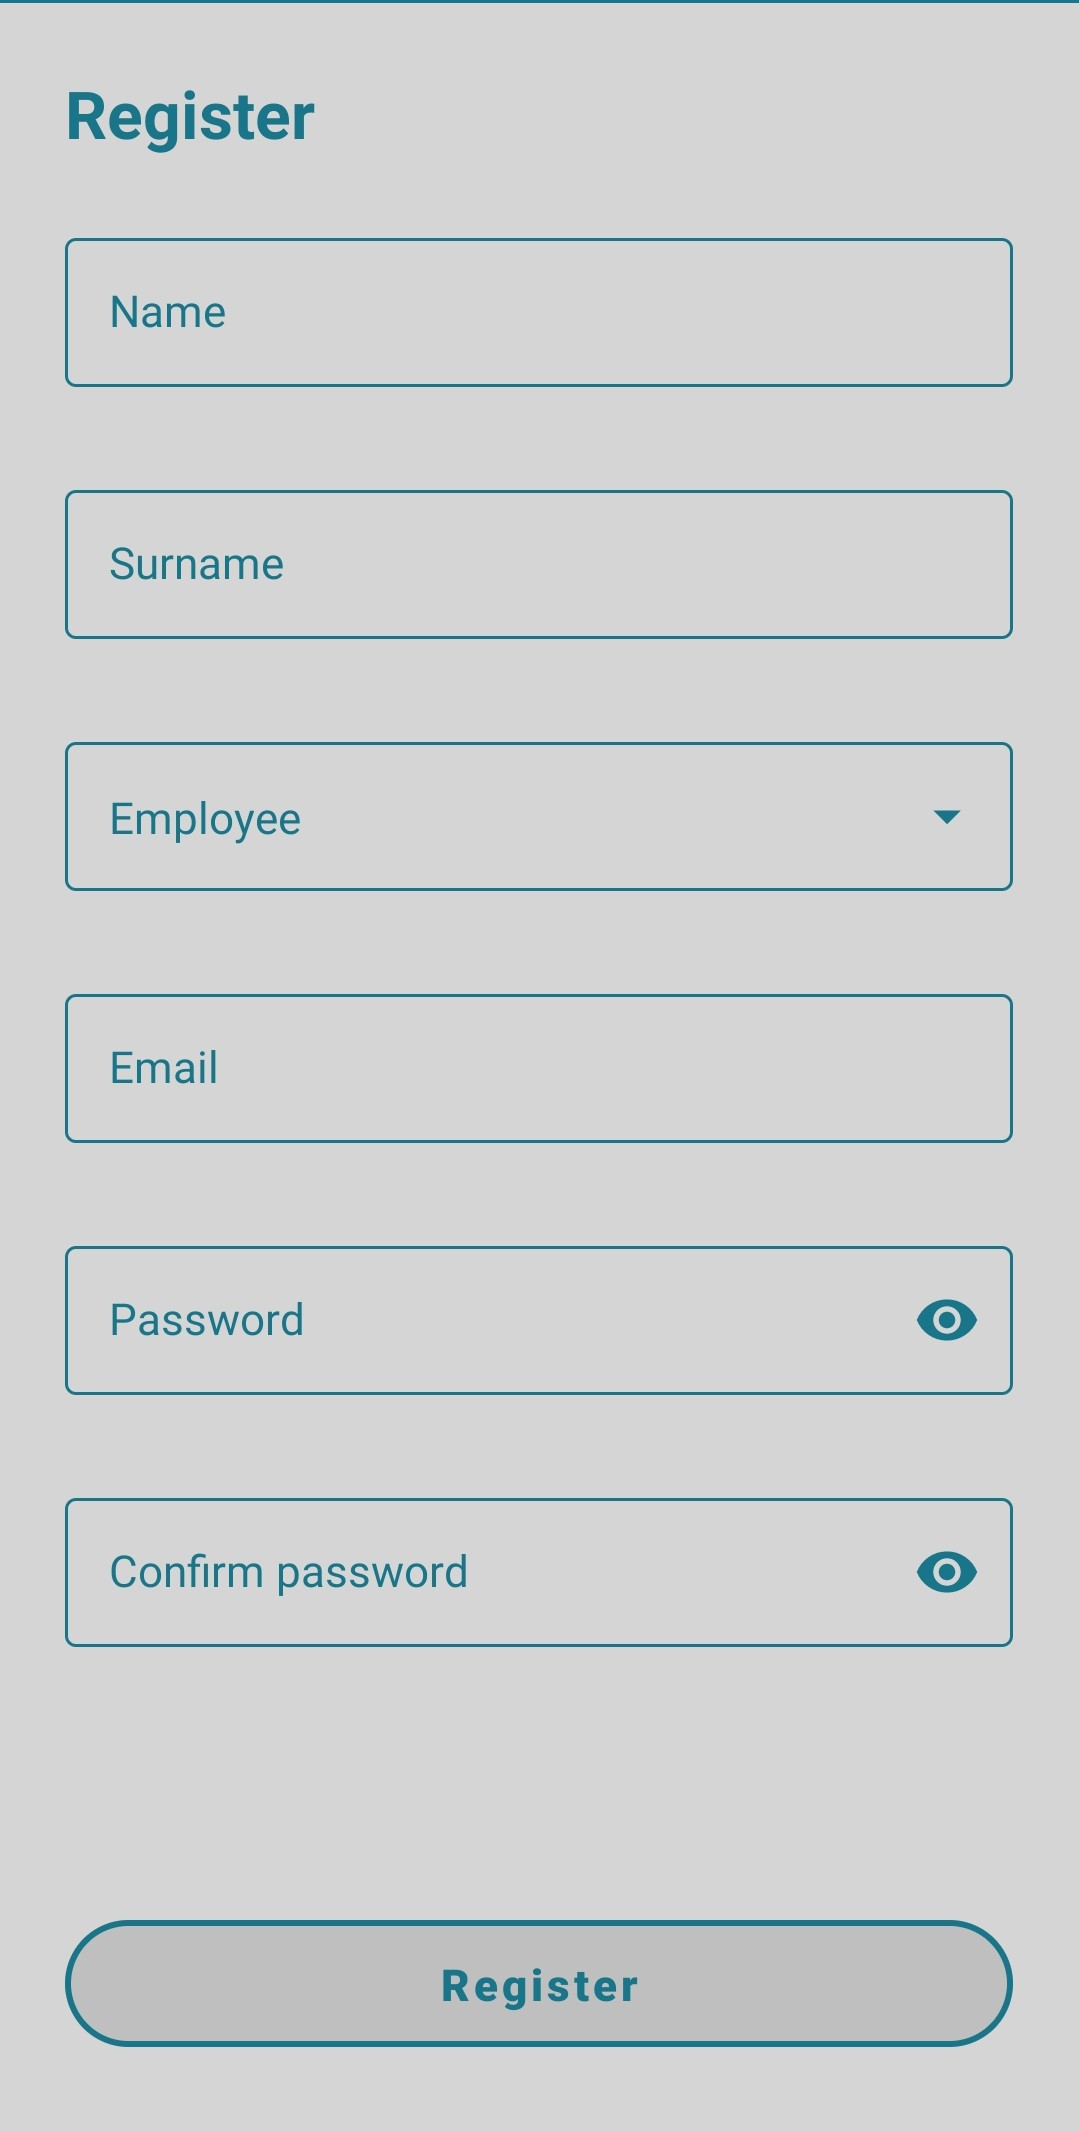
\includegraphics[scale=0.25]{slike/register.jpg}
				\caption{Zaslon za registraciju}
			\end{figure}
			
			\eject 
		
		
		\section{Dijagram razmještaja}
			
			 	\justify{Dijagram razmještaja je strukturni statički UML dijagram koji opisuje topologiju sustava i usredotočen je na odnos sklopovskih i programskih dijelova. Na slici 5.7 prikazan je specifikacijski dijagram razmještaja. Specifikacijski dijagram prikazuje pregled implementacije artefakata bez upućivanja na specifične slučajeve artefakata ili čvorova. Na poslužiteljskom računalu se nalazi poslužitelj baze podataka. Klijent koristi mobilnu aplikaciju namijenjenu za operacijski sustav Android. Komunikacija između klijenta i baze podataka odvija se preko protokola HTTP.}\\
			 
			 \begin{figure}[H]
			 	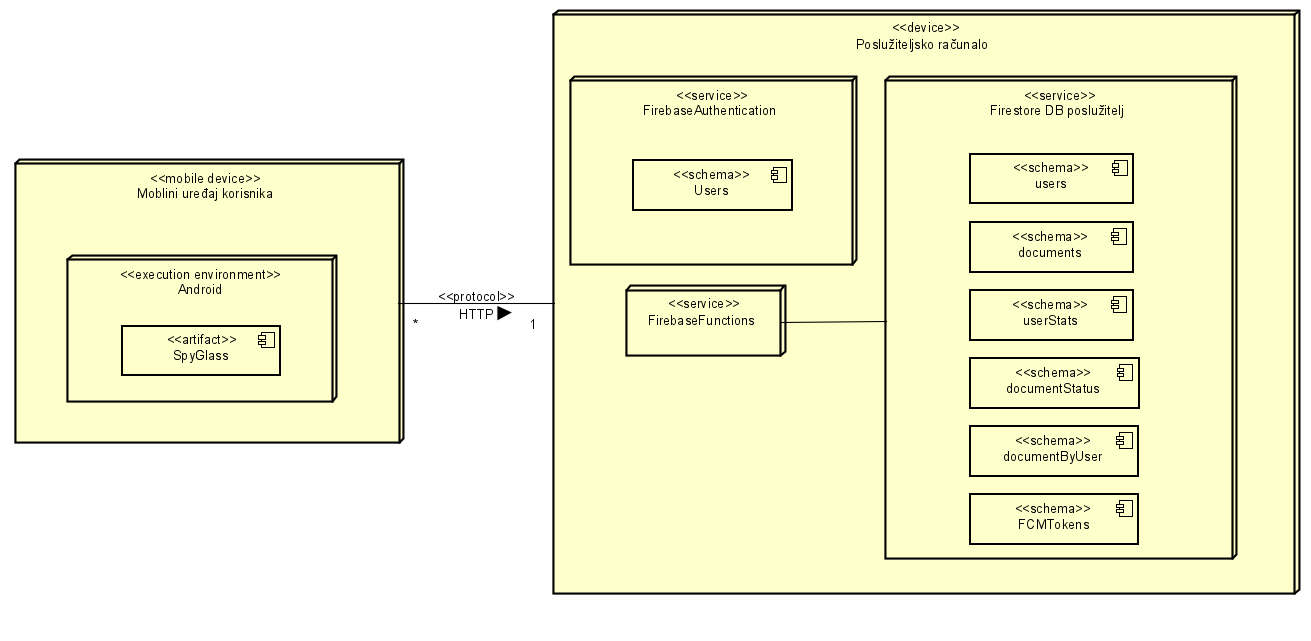
\includegraphics[width=\textwidth]{slike/Dijagram_razmjestaja.png}
			 	\caption{Dijagram razmještaja}
			 \end{figure}
			
			\eject 
		
		\section{Upute za puštanje u pogon}

		\subsection{Kreiranje projekta i integracija SDK-a u Android}
		\begin{packed_enum}
			\item Kreirati Firebase projekt
				\begin{packed_enum}
					\item Imenovati projekt
					\item Omogućiti \textbf{Google Analytics}
					\item Kliknuti \textbf{Create project}
				\end{packed_enum}
	
			\item Registrirati aplikaciju
				\begin{packed_enum}
					\item Kliknuti opciju \textbf{Add app}
					\item Unijeti Android package name koji odgovara imenu od aplikacije
					\item Kliknuti \textbf{Register app}
				\end{packed_enum}
	
			\item Dodati Firebase configuration datoteku u aplikaciju
				 \begin{packed_enum}
					\item Preuzeti \textbf{google-services.json} iz Firebase konzole
					\item Staviti datoteku u ispravni direktorij (module ili app-level direktorij)
					\item Dodati u \textbf{build.gradle} datoteku koja se nalazi u root-level ili project-level direktoriju navedeni tekst:
						\begin{lstlisting}[mathescape=true,breaklines=true,autogobble=true]
							buildscript {
	
								repositories {
									// Check that you have the following line (if not, add it):
									google()  // Google's Maven repository
								}
	
								dependencies {
									// ...
	
									// Add the following line:
									classpath 'com.google.gms:google-services:4.3.10'  // Google Services plugin
								}
							}
	
								allprojects {
								// ...
	
									repositories {
										// Check that you have the following line (if not, add it):
										google()  // Google's Maven repository
										// ...
									}
								}
						\end{lstlisting}
					\item Dodati u \textbf{build.gradle} datoteku koja se nalazi u module ili app-level direktoriju navedeni tekst:
						\begin{lstlisting}[mathescape=true,breaklines=true,autogobble=true]
							apply plugin: 
							'com.android.application'
							// Add the following line:
							apply plugin: 'com.google.gms.google-services'  // Google Services plugin
	
							android {
							// ...
						}
						\end{lstlisting}
				\end{packed_enum}
	
			\item Dodati Firebase SDK u aplikaciju
				\begin{packed_enum}   
					\item Dodati u \textbf{build.gradle} datoteku koja se nalazi u module ili app-level direktoriju navedeni tekst:      
						\begin{lstlisting}[mathescape=true,breaklines=true,autogobble=true]
							dependencies {
							// ...
				  
							// Import the Firebase BoM
							implementation platform('com.google.firebase:firebase-bom:29.0.3')
				  
							// When using the BoM, you don't specify versions in Firebase library dependencies
				  
							// Declare the dependency for the Firebase SDK for Google Analytics
							implementation 'com.google.firebase:firebase-analytics-ktx'
				  
							// Declare the dependencies for any other desired Firebase products
							// For example, declare the dependencies for Firebase Authentication and Cloud Firestore
							implementation 'com.google.firebase:firebase-auth-ktx'
							implementation 'com.google.firebase:firebase-firestore-ktx'
						  }
						\end{lstlisting} 
					\item Kliknuti gumb \textbf{Sync} u programu Android Studio kako bi svi \textbf{dependencies} bili na najnovijoj verziji
				\end{packed_enum} 
	
			\item U Firebase konzoli omogućiti authentifikaciju preko email adrese i lozinke
				\begin{packed_enum}
					\item Otvoriti \textbf{Auth} sekciju unutar konzole
					\item Pod \textbf{Sign in method} odabrati opciju \textbf{Email/password} i kliknuti gumb \textbf{Save}
				\end{packed_enum}
	
			\item Dodati \textbf{dependencies} za Firebase authentifikaciju
				\begin{packed_enum}
					\item Dodati u \textbf{build.gradle} datoteku koja se nalazi u module ili app-level direktoriju navedeni tekst:
					\begin{lstlisting}[mathescape=true,breaklines=true,autogobble=true]
						dependencies {
							// Import the BoM for the Firebase platform
							implementation platform('com.google.firebase:firebase-bom:29.0.3')
				
							// Declare the dependency for the Firebase Authentication library
							// When using the BoM, you don't specify versions in Firebase library dependencies
							implementation 'com.google.firebase:firebase-auth-ktx'
						}
					\end{lstlisting}
				\end{packed_enum}
		\end{packed_enum}	 
		
		\subsection{Puštanje u pogon Cloud Funkcija}
		\justify{
			\textbf{Cloud Functions} služe za automatsko pokretanje pozadinskog koda kao odgovor na događaje koje pokreću značajke Firebasea, primjerice triggeri kolekcija u bazi podataka. 
		Nakon kreiranja Firebase projekta, opisanog u prethodnom dijelu teksta potrebni su sljedeći koraci:}
		\begin{packed_enum}
			\item Instalacija node.js i Firebase CLI-a. Potrebno je instalirati i npm, te pokrenuti sljedeću naredbu:
				\begin{lstlisting}[mathescape=true,breaklines=true,autogobble=true]
					npm install -g firebase-tools
				\end{lstlisting}
			\item Povezati projekt lokalno s cloudom:
				\begin{lstlisting}[mathescape=true,breaklines=true,autogobble=true]
					firebase login
					firebase init firestore
					firebase init functions
				\end{lstlisting}
			\item Napisati Cloud funkciju te pokrenuti
				\begin{lstlisting}[mathescape=true,breaklines=true,autogobble=true]
					firebase deploy --only functions
				\end{lstlisting}
		\end{packed_enum}

		\subsection{Pokretanje Android aplikacije}
		\justify{Potrebno je preuzeti spyglass.apk datoteku s Gitlab repozitorija projekta pod direktorijem \textit{apk} na mobilni uređaj. 
		Zatim ju je potrebno pokrenuti čime će se pokrenuti i instalacija Android aplikacije nakon čega klikom na ikonu aplikacije
		pokrećemo aplikaciju.}
			
			\eject 